% \documentclass[aspectratio=169, 11pt]{beamer}
\documentclass[aspectratio=169, 11pt, handout]{beamer}

% ── Theme ──
\usetheme{Madrid}
\usecolortheme{default}
\setbeamertemplate{navigation symbols}{}
\setbeamertemplate{footline}{%
  \leavevmode\hbox{%
    \begin{beamercolorbox}[wd=.333333\paperwidth,ht=2.5ex,dp=1ex,center]{author in head/foot}%
      \usebeamerfont{author in head/foot}\insertshortauthor
    \end{beamercolorbox}%
    \begin{beamercolorbox}[wd=.333333\paperwidth,ht=2.5ex,dp=1ex,center]{title in head/foot}%
      \usebeamerfont{title in head/foot}\insertshorttitle
    \end{beamercolorbox}%
    \begin{beamercolorbox}[wd=.333333\paperwidth,ht=2.5ex,dp=1ex,right]{date in head/foot}%
      \usebeamerfont{date in head/foot}\insertframenumber{} / \inserttotalframenumber\hspace*{2ex}
    \end{beamercolorbox}}}

% ── Packages ──
\usepackage{amsmath,amssymb}
\usepackage{booktabs}
\usepackage{xcolor}
\usepackage{colortbl}
\usepackage{graphicx}
\usepackage{tikz}
\usetikzlibrary{arrows.meta, positioning, calc}

% ── Colors ──
\definecolor{sbgreen}{HTML}{00704A}  % course accent
\definecolor{warnred}{HTML}{CC0000}
\definecolor{noteblue}{HTML}{2060A0}

% ── Commands ──
\newcommand{\E}{\mathbb{E}}
\newcommand{\Var}{\mathrm{Var}}
\newcommand{\Cov}{\mathrm{Cov}}
\newcommand{\SE}{\mathrm{SE}}
\newcommand{\Prob}{\mathrm{Pr}}
\newcommand{\indep}{\perp\!\!\!\perp}

\usepackage{soul}
\newcommand{\NUM}[2]{\sethlcolor{yellow}\hl{#1\,\textsuperscript{?}}\marginpar{\tiny #2}}
% Beamer frames are typeset inside boxes, where \marginpar raises "Not in outer par mode"
% and \marginparwidth is 4pt. Same marker; the provenance note goes to the frame footnote.
\renewcommand{\NUM}[2]{\sethlcolor{yellow}\hl{#1\,\textsuperscript{?}}\footnote[frame]{\tiny #2}}
% Compact footnote layout so several provenance notes fit under one frame.
\setbeamertemplate{footnote}{\noindent\raggedright\hspace*{0.6em}\tiny\insertfootnotemark\,\insertfootnotetext\par}
% TikZ styles used by the frames carried verbatim from old-decks/lecture06.tex (copied from its preamble).
\tikzset{
    tnode/.style={draw, rounded corners, fill=gray!10, minimum width=2.2cm, minimum height=0.65cm, font=\small, align=center},
    tgreen/.style={tnode, fill=sbgreen!15, draw=sbgreen},
    tblue/.style={tnode, fill=noteblue!12, draw=noteblue},
    tred/.style={tnode, fill=red!8, draw=warnred},
    tarrow/.style={-{Stealth}, thick}
}

% Version 2 (2026-09-29). Course spine: estimand -> identification -> estimation.
% Changes from slides.tex: m06/CHANGES-v2.md.
\newcommand{\spinestep}[1]{\textcolor{sbgreen}{\textbf{#1}}}

% ── Title ──
\title[Meeting 6]{Meeting 6: Caps, Budgets and Spending Risk}
\subtitle{Applied Causal Inference for Business}
\author{Zhikun Lu}
\date{\today}

\begin{document}

% ====================================================================
\begin{frame}
\titlepage
\end{frame}

% ====================================================================
\begin{frame}{Where Does the Counterfactual Come From?}

\begin{center}
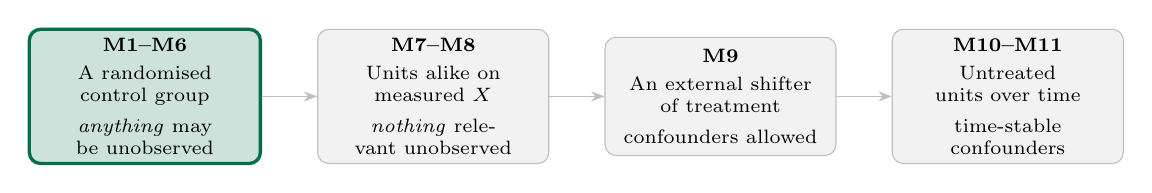
\begin{tikzpicture}[
    node distance=0.45cm and 0.7cm,
    box/.style={draw, rounded corners, minimum width=2.9cm, minimum height=1.5cm,
                font=\scriptsize, align=center, text width=2.7cm},
    active/.style={box, fill=sbgreen!20, draw=sbgreen, very thick},
    inactive/.style={box, fill=gray!10, draw=gray!50}
]
\node[active] (A) {\textbf{M1--M6}\\[2pt] A randomised control group\\[3pt] \emph{anything} may be unobserved};
\node[inactive, right=of A] (B) {\textbf{M7--M8}\\[2pt] Units alike on measured $X$\\[3pt] \emph{nothing} relevant unobserved};
\node[inactive, right=of B] (C) {\textbf{M9}\\[2pt] An external shifter of treatment\\[3pt] confounders allowed};
\node[inactive, right=of C] (D) {\textbf{M10--M11}\\[2pt] Untreated units over time\\[3pt] time-stable confounders};

\draw[-{Stealth}, gray!50] (A) -- (B);
\draw[-{Stealth}, gray!50] (B) -- (C);
\draw[-{Stealth}, gray!50] (C) -- (D);
\end{tikzpicture}
\end{center}

\bigskip

\begin{center}
\small The last meeting of the first box. The effects are identified and evaluated;\\
today the constraints the business actually operates under decide who gets treated.
\end{center}
\end{frame}

% ====================================================================
\begin{frame}{Today's Plan}

\begin{center}
\small
\begin{tabular}{rll}
\toprule
\textbf{Minutes} & \textbf{Block} & \\
\midrule
0--60 & A & \textbf{Exam I} (M1--M5) \\
70--120 & B & From effects to a list: costs, caps, budgets, spending risk \\
130--180 & C & \textbf{Lab 3:} tool calling over experiment records and statistical functions \\
\bottomrule
\end{tabular}
\end{center}

\bigskip

\textbf{Block B, on the spine:}
\begin{enumerate}\small
    \item \spinestep{Estimand:} the net value of a list under the business's constraints
    \item \spinestep{Identification:} the push test's coin, and transport to Q4
    \item \spinestep{Estimation, then decision:} a threshold, a cap, costs that differ, a budget and its shadow price, spending risk, noisy estimates
\end{enumerate}

\bigskip

\textbf{Case:} Lin's coupon programme, Meeting 6 (Releases 1--3). \quad \textbf{At home:} the targeting core, with Notebook 6 (72 hours). \quad \textbf{Due 72 hours before M7:} project proposal.
\end{frame}

% ====================================================================
\begin{frame}{Exam I: M1--M5}

\begin{center}
\begin{tabular}{rl}
\toprule
0--3 & Instructions and questions about the paper \\
3--58 & \textbf{55 minutes} of work \\
58--60 & Papers collected; break until 70 \\
\bottomrule
\end{tabular}
\end{center}

\bigskip

\textbf{Examinable:} the slides of M1--M5 and Section~1 of each set of notes. Section~3 of the notes and anything marked \emph{Extension} are not.

\bigskip

\textbf{The one habit that earns marks:} in every question, find the \emph{number that decides it} before computing anything, and say which comparison produced it.
\end{frame}

% ====================================================================
\section{The Estimand and Its Identification: The Q4 Push}
% ====================================================================

% [RELEASE R1 — the Q4 push and the Region 2 push test]
\begin{frame}{The Q4 Push}

Marketing wants to reach Region 2 in Q4 with something cheaper than M1's \textyen 10 coupon: an \textbf{app push notification} carrying a \textyen 5-off coupon for a seasonal drink.

\bigskip

A two-week push test in Region 2 (50/50 within every cell, 10{,}000 members) gave the M4 pattern again:

\begin{center}
\small
\begin{tabular}{llccc}
\toprule
\textbf{Type} & \textbf{Spending} & $\hat{\tau}(x)$ & \textbf{Count} & \textbf{Share} \\
\midrule
Analyst   & High & 20\% & 2,500 & 25\% \\
Analyst   & Low  & 20\% & 2,500 & 25\% \\
Executive & High & 5\%  & 2,500 & 25\% \\
Executive & Low  & 5\%  & 2,500 & 25\% \\
\bottomrule
\end{tabular}
\end{center}

\bigskip

\textbf{Question:} who gets the push? Each purchase it causes earns $m = $ \textyen 30 of margin.
\end{frame}

% ====================================================================
\begin{frame}{The Number That Decides It}

Every member on the list earns the purchases the push causes and costs whatever the push costs:
\[
v_i \;=\; \underbrace{\hat\tau(x_i) \cdot 30}_{\text{margin on caused purchases}} \;-\; \underbrace{\hat c(x_i)}_{\text{everything the push costs}}
\]

\pause

\begin{alertblock}{The list}
\[
\max_{d_1, \ldots, d_n \in \{0,1\}} \; \sum_i d_i\, v_i \qquad \text{subject to whatever the business imposes}
\]
\end{alertblock}

\bigskip

Every step today adds \textbf{one cost or one constraint}. The effects $\hat\tau(x)$ never change. The list does --- and so does the reason each member is on it or off it.

\medskip

Hold the analyst--low and analyst--high rows side by side. They have the same effect. Watch when they stop being interchangeable.
\end{frame}

% ====================================================================
\begin{frame}{What Must Be True}

From the push test's log and the Q4 plan:

\bigskip

\begin{center}
\small
\begin{tabular}{p{6.4cm}p{6.6cm}}
\toprule
\textbf{The case says} & \textbf{Which buys} \\
\midrule
``The push test drew 50/50 within every type $\times$ spending cell.'' & $\hat\tau(x)$ identified cell by cell (M1, M3). \\[0.4em]
``Q4 sends the same push, the same \textyen 5 coupon, to the same members.'' & The test's effects transport to the decision (M2). \\[0.4em]
``Each member receives at most one push; the coupon is single-use.'' & No interference: each $v_i$ can be computed on its own and the $v_i$ add up. \\
\bottomrule
\end{tabular}
\end{center}

\bigskip
\pause

The third sentence is the one this lecture leans on hardest. Every optimisation today is a \textbf{sum} of member-level values. We come back to when it fails.
\end{frame}

% ====================================================================
\section{From Estimates to a List: Costs and Caps}
% ====================================================================

% [CARRIED VERBATIM from old-decks/lecture06.tex:149]
\begin{frame}{Step 1: Zero-Cost Treatment}

Suppose, for now, that the push and its coupon cost nothing: ignore redemptions and opt-outs. (A push \emph{without} the coupon would be a different treatment, whose effects the test never measured.)\\

\medskip

If sending the notification costs nothing, the decision rule is trivial:
\[
d^*(x_i) = \mathbf{1}\{\hat{\tau}(x_i) > 0\}
\]

\pause

\begin{center}
\begin{tabular}{llccc}
\toprule
\textbf{Type} & \textbf{Spending} & $\hat{\tau}(x)$ & $\hat{\tau} > 0$? & \textbf{Notify?} \\
\midrule
Analyst & High & 20\% & \textcolor{sbgreen}{Yes} & \textcolor{sbgreen}{Yes} \\
Analyst & Low & 20\% & \textcolor{sbgreen}{Yes} & \textcolor{sbgreen}{Yes} \\
Executive & High & 5\% & \textcolor{sbgreen}{Yes} & \textcolor{sbgreen}{Yes} \\
Executive & Low & 5\% & \textcolor{sbgreen}{Yes} & \textcolor{sbgreen}{Yes} \\
\bottomrule
\end{tabular}
\end{center}

\bigskip

All 10,000 customers get notified. Every customer is evaluated independently.

\end{frame}

% [CARRIED VERBATIM from old-decks/lecture06.tex:183]
\begin{frame}{Step 2: A Hidden Cost}

The data science team discovers: some notified customers \textbf{disable notifications permanently}.

\medskip

\begin{itemize}
    \item Long-term revenue loss from opt-out: \textyen150. Opt-out probability: $p_{\text{opt}} = 1\%$.
    \item Expected cost per notification: $c = 150 \times 0.01 = \text{\textyen}1.50$.
\end{itemize}

\pause
\medskip

Revenue per incremental visit: $m = \text{\textyen}30$. Threshold: $c/m = 1.50/30 = 5\%$.
\[
d^*(x_i) = \mathbf{1}\left\{\hat{\tau}(x_i) > 5\%\right\}
\]

\pause
\medskip

\begin{center}
\begin{tabular}{llccc}
\toprule
\textbf{Type} & \textbf{Spending} & $\hat{\tau}(x)$ & $\hat{\tau} > 5\%$? & \textbf{Notify?} \\
\midrule
Analyst & High/Low & 20\% & \textcolor{sbgreen}{Yes} & \textcolor{sbgreen}{Yes (5,000)} \\
Executive & High/Low & 5\% & \textcolor{warnred}{Borderline} & \textcolor{warnred}{No} \\
\bottomrule
\end{tabular}
\end{center}

\end{frame}

% [CARRIED VERBATIM from old-decks/lecture06.tex:220]
\begin{frame}{Step 3: Budget Constraint}

The data science team also discovers that if we send notifications at a low frequency, the opt-out rate would be significantly lower. Therefore, the product management caps notifications at \textbf{1,000 per day} to limit notification fatigue.

\bigskip

Even if all analysts pass the threshold, only 1,000 can be notified. Customers now \emph{compete}.

\pause
\bigskip

\begin{center}
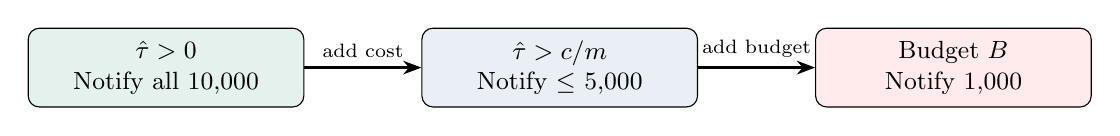
\begin{tikzpicture}[
    block/.style={draw, rounded corners, minimum width=3.5cm, minimum height=1cm, font=\small, align=center}
]
\node[block, fill=sbgreen!10] (s1) at (0,0) {$\hat{\tau} > 0$\\Notify all 10,000};
\node[block, fill=noteblue!10] (s2) at (5,0) {$\hat{\tau} > c/m$\\Notify $\leq$ 5,000};
\node[block, fill=red!8] (s3) at (10,0) {Budget $B$\\Notify 1,000};
\draw[tarrow] (s1) -- (s2) node[midway, above, font=\scriptsize]{add cost};
\draw[tarrow] (s2) -- (s3) node[midway, above, font=\scriptsize]{add budget};
\end{tikzpicture}
\end{center}

\bigskip

Each step adds one friction. The marginal customer is no longer evaluated against zero or a fixed threshold; they are evaluated against the \emph{next best alternative}.

\end{frame}

% [CARRIED VERBATIM from old-decks/lecture06.tex:255]
\begin{frame}{The Budget-Constrained Problem}

At this stage, cost $c = \text{\textyen}1.50$ is \textbf{uniform} across customers (same opt-out risk for everyone).

\begin{block}{Optimization}
\vspace{-0.5em}
\[
\max_{d_1, \ldots, d_n \in \{0,1\}} \sum_{i=1}^{n} d_i \cdot \bigl[\hat{\tau}(x_i) \cdot m - c\bigr] \qquad \text{subject to} \quad \sum_{i=1}^{n} d_i \leq B
\]
\end{block}

\pause
\bigskip

The objective is \textbf{separable} in $d_i$. The solution is sorting:

\begin{enumerate}
    \item Compute net value: $v_i = \hat{\tau}(x_i) \cdot m - c$ for each customer.
    \item Rank by $v_i$ in decreasing order.
    \item Treat the top $\min(B,\; |\{i : v_i > 0\}|)$ customers.
\end{enumerate}

\pause
\bigskip

When cost is uniform, ranking by $v_i$ is the same as ranking by $\hat{\tau}(x_i)$.


\small \textbf{Why sorting is optimal:} if a list holds $b$ but not $a$, with $v_a > v_b$, swapping them keeps the count and raises the value. Repeat until no swap helps. If fewer than $B$ values are positive, leave slots empty: a cap is an upper bound, not a quota.
\end{frame}

% ====================================================================
\begin{frame}{Region 2: A Cap of 1{,}000 Notifications}

Uniform cost \textyen 1.50: every analyst has $v_i = 0.20 \times 30 - 1.50 = $ \textyen 4.50, every executive \textyen 0. \textbf{The card cannot rank 5{,}000 analysts for 1{,}000 slots:} any 1{,}000 of them earn \textyen 4{,}500.

\pause
\medskip

Suppose the M4 forest's member-level estimates split the analysts three ways (averaging $0.20$, as the card does):

\begin{center}
\small
\begin{tabular}{lrcrl}
\toprule
\textbf{Forest group} & \textbf{Members} & $\hat{\tau}(x)$ & $v_i = \hat{\tau} \cdot 30 - 1.50$ & \textbf{Notify?} \\
\midrule
Top analysts & 1{,}000 & 0.30 & \textyen 7.50 & \textcolor{sbgreen}{Yes (all 1{,}000)} \\
Middle analysts & 2{,}000 & 0.20 & \textyen 4.50 & \textcolor{warnred}{No (cap)} \\
Other analysts & 2{,}000 & 0.15 & \textyen 3.00 & \textcolor{warnred}{No (cap)} \\
\bottomrule
\end{tabular}
\end{center}

\small Check: $(1{,}000 \times 0.30 + 2{,}000 \times 0.20 + 2{,}000 \times 0.15)/5{,}000 = 0.20$.

\pause
\normalsize
Under the cap the forest's list earns \textyen 7{,}500. \textbf{The constraint, not the threshold, binds} --- and it makes ranking \emph{within} a segment worth money.
\end{frame}

% ====================================================================
\section{Costs That Differ}
% ====================================================================

% [RELEASE R2 — push-test purchase rates by cell with and without the push; the coupon is paid on redemption]
% [CARRIED VERBATIM from old-decks/lecture06.tex:322]
\begin{frame}{Why Costs Are Not Uniform}
 
So far: every notification costs the same (\textyen1.50 opt-out risk). But the \textyen5 coupon creates an additional cost that varies by customer.
 
\pause
\smallskip
 
\textbf{Key insight:} the coupon is redeemed only upon purchase, so:
\vspace{-0.5em}
\[
\hat{c}(x_i) = \underbrace{1.50}_{\text{opt-out}} + \underbrace{5 \times \Prob(Y(1)\!=\!1 \mid X_i)}_{\text{expected coupon payout}} \qquad v_i = \hat{\tau}(x_i) \cdot m - \hat{c}(x_i)
\]
\vspace{-0.8em}
 
\pause
 
\begin{center}
\small
\begin{tabular}{llcccccl}
\toprule
\textbf{Type} & \textbf{Spend} & $\hat{\tau}$ & $\Prob(Y_0\!=\!1)$ & $\Prob(Y_1\!=\!1)$ & $\hat{c}(x)$ & $v_i$ & \textbf{Treat?} \\
\midrule
Analyst & Low  & 20\% & 0\% & 20\% & \textyen2.50 & \textyen3.50 & \textcolor{sbgreen}{Yes} \\
Analyst & High & 20\% & 30\% & 50\% & \textyen4.00 & \textyen2.00 & \textcolor{sbgreen}{Yes} \\
Exec & Low  & 5\% & 30\% & 35\% & \textyen3.25 & $-$\textyen1.75 & \textcolor{warnred}{No} \\
Exec & High & 5\% & 60\% & 65\% & \textyen4.75 & $-$\textyen3.25 & \textcolor{warnred}{No} \\
\bottomrule
\end{tabular}
\end{center}
 
\pause
\smallskip
 
Under \textbf{uniform cost}, spending was irrelevant. Under \textbf{heterogeneous cost}, all four segments separate: high baseline $\Prob(Y_0\!=\!1)$ drives up cost.
 
\end{frame}

% [CARRIED VERBATIM from old-decks/lecture06.tex:361]
\begin{frame}{Why Are High Spenders Expensive?}
 
The same net value admits a revealing decomposition:
\vspace{-0.8em}
\[
v_i = \underbrace{\hat{\tau}(x_i) \cdot (m - 5)}_{\substack{\text{incremental buyers:}\\\text{margin minus coupon}}} \;-\; \underbrace{5 \cdot \Prob(Y(0)\!=\!1 \mid X_i)}_{\substack{\text{baseline buyers:}\\\text{coupon, no new revenue}}} \;-\; 1.50
\]
\vspace{-1.0em}
 
\pause
 
The second term is the \textbf{sure-thing cost}: customers who would have purchased anyway redeem the coupon for free.
 
\smallskip
 
\begin{center}
\small
\begin{tabular}{llcccc}
\toprule
\textbf{Type} & \textbf{Spend} & $\hat{\tau}\!\cdot\!25$ & $5 \!\times\! \Prob(Y_0\!=\!1)$ & $- 1.50$ & $v_i$ \\
\midrule
Analyst & Low  & \textyen5.00 & \textyen0.00 & $-$\textyen1.50 & \textyen3.50 \\
Analyst & High & \textyen5.00 & \textyen1.50 & $-$\textyen1.50 & \textyen2.00 \\
Executive & Low  & \textyen1.25 & \textyen1.50 & $-$\textyen1.50 & $-$\textyen1.75 \\
Executive & High & \textyen1.25 & \textyen3.00 & $-$\textyen1.50 & $-$\textyen3.25 \\
\bottomrule
\end{tabular}
\end{center}
\vspace{-0.5em}
 
\pause
 
Analyst-Low has zero sure-thing cost (nobody buys without the coupon). Analyst-High loses \textyen1.50 to baseline buyers. Same CATE, different profitability.
 
\pause
\vspace{0.2em}
 
\textbf{Note:} $\hat{c}(x_i) = 1.50 + 5 \!\times\! \Prob(Y(1)\!=\!1)$ gives the same $v_i$. The two formulas are algebraically equivalent; use whichever builds the right intuition.
 
\end{frame}

% [CARRIED VERBATIM from old-decks/lecture06.tex:405]
\begin{frame}{The Two-Model Pipeline}
 
With customer-heterogeneous costs, targeting requires \textbf{two} ML models:
 
\bigskip
 
\begin{enumerate}
    \item \textbf{Benefit model} (causal): estimate $\hat{\tau}(x_i)$ from the experiment.
    
    Requires counterfactual reasoning (M1--M5).
    
    \medskip
    
    \item \textbf{Cost model} (predictive): estimate $\hat{c}(x_i)$ from past campaign data.
    
    Standard supervised learning: predict $\Prob(Y(1)\!=\!1 \mid X)$ from treated observations. Or equivalently, predict $\Prob(Y(0)\!=\!1 \mid X)$ from control observations, then add $\hat{\tau}(x_i)$.
\end{enumerate}
 
\pause
\bigskip
 
The causal/predictive distinction matters:
\begin{itemize}
    \item Benefit side requires experimental or quasi-experimental data.
    \item Cost side can use observational data from past campaigns.
\end{itemize}
 
\pause
\bigskip
 
Different estimation tasks, different data requirements.
 
\end{frame}

% [CARRIED VERBATIM from old-decks/lecture06.tex:441]
\begin{frame}{Without a Budget: Customer-Specific Thresholds}
 
With no budget constraint, each customer is evaluated independently, but the threshold is now \emph{customer-specific}:
\[
d^*(x_i) = \mathbf{1}\bigl\{\hat{\tau}(x_i) \cdot m > \hat{c}(x_i)\bigr\}
\]
 
\pause
\bigskip
 
\begin{center}
\begin{tabular}{llccccl}
\toprule
\textbf{Type} & \textbf{Spend} & $\hat{\tau}$ & $\hat{\tau}\!\cdot\!30$ & $\hat{c}(x)$ & Net & \textbf{Treat?} \\
\midrule
Analyst & Low  & 20\% & \textyen6.00 & \textyen2.50 & \textyen3.50 & \textcolor{sbgreen}{Yes} \\
Analyst & High & 20\% & \textyen6.00 & \textyen4.00 & \textyen2.00 & \textcolor{sbgreen}{Yes} \\
Executive & Low  & 5\% & \textyen1.50 & \textyen3.25 & $-$\textyen1.75 & \textcolor{warnred}{No} \\
Executive & High & 5\% & \textyen1.50 & \textyen4.75 & $-$\textyen3.25 & \textcolor{warnred}{No} \\
\bottomrule
\end{tabular}
\end{center}
 
\pause
\bigskip
 
Both analyst segments pass; both executive segments fail. But the \textbf{net values differ}: Analyst-Low generates \textyen3.50 per customer vs.\ Analyst-High at \textyen2.00. The prognostic variable now matters for ranking.
 
\end{frame}

% [CARRIED VERBATIM from old-decks/lecture06.tex:473]
\begin{frame}[shrink=7]{How Much Will the Campaign Cost?}
 
The firm treats all 5,000 analysts. Expected total cost:
\[
\hat{\mu}_C = 2{,}500 \times 4.00 + 2{,}500 \times 2.50 = \text{\textyen}16{,}250
\]
 
\pause
\medskip
 
But realized cost is random. Each customer either redeems (\textyen6.50) or not (\textyen1.50). If redemption runs higher than predicted, actual cost exceeds the estimate.
 
\pause
\medskip
 
Finance asks: ``What is the chance we exceed \textyen18,000?''
 
\medskip
 
Under a normal approximation for total cost:
\[
\Prob\!\left(\sum_{i} d_i \cdot c_i > C\right) \leq \alpha \quad \Longleftrightarrow \quad \hat{\mu}_C + z_\alpha \hat{\sigma}_C \leq C
\]
 
\pause
\medskip
 
Even without a hard budget cap, the firm wants to control spending risk. The safety margin $z_\alpha \hat{\sigma}_C$ gives finance a confidence interval on total campaign cost.
 

\small \textbf{The answer for finance.} With independent redemptions, $\hat\sigma_C = \sqrt{2{,}500(25)(0.16) + 2{,}500(25)(0.25)} = \text{\textyen}160$, so $z = (18{,}000 - 16{,}250)/160 = 10.9$: \textbf{essentially zero}. The 95th percentile of cost is $16{,}250 + 1.645(160) = \text{\textyen}16{,}513$. Common demand shocks and estimated redemption rates make the real risk larger than this.
\end{frame}

% ====================================================================
\section{Budgets}
% ====================================================================

% [RELEASE R3 — finance's memo: \textyen 8,000 of expected cost, at most 5% chance of overrun]
% [CARRIED VERBATIM from old-decks/lecture06.tex:506]
\begin{frame}{With a Budget: The Knapsack Problem}
 
Now finance imposes a hard cap: total campaign cost $\leq C$.
 
\bigskip
 
With heterogeneous costs, this is a \textbf{knapsack}:
\[
\max_{d_1, \ldots, d_n} \sum_{i=1}^{n} d_i \cdot \hat{\tau}(x_i) \cdot m \qquad \text{subject to} \quad \sum_{i=1}^{n} d_i \cdot \hat{c}(x_i) \leq C
\]
 
\pause
\bigskip
 
The greedy solution --- exact here, because each cell holds 2{,}500 interchangeable members --- ranks by the \textbf{benefit-cost ratio}:
\[
r_i = \frac{\hat{\tau}(x_i) \cdot m}{\hat{c}(x_i)}
\]
and treat in decreasing order of $r_i$ until the budget is exhausted.
 
\pause
\bigskip
 
With uniform costs, ranking by $r_i$ reduces to ranking by $\hat{\tau}(x_i)$, so spending was irrelevant. With heterogeneous costs, spending enters through $\hat{c}(x_i)$ and changes the ranking.
 
\end{frame}

% ====================================================================
\begin{frame}{Knapsack: Region 2 Numerics}

\begin{center}
\begin{tabular}{llccccc}
\toprule
\textbf{Type} & \textbf{Spend} & $\hat{\tau}$ & $\hat{\tau}\!\cdot\!30$ & $\hat{c}(x)$ & $r_i$ & \textbf{Rank} \\
\midrule
Analyst & Low  & 20\% & \textyen6.00 & \textyen2.50 & 2.40 & \textcolor{sbgreen}{1st} \\
Analyst & High & 20\% & \textyen6.00 & \textyen4.00 & 1.50 & 2nd \\
Executive & Low  & 5\% & \textyen1.50 & \textyen3.25 & 0.46 & 3rd \\
Executive & High & 5\% & \textyen1.50 & \textyen4.75 & 0.32 & 4th \\
\bottomrule
\end{tabular}
\end{center}

\pause
\medskip

\textbf{Finance's cap: \textyen 8{,}000 of expected cost.} Fill in order of $r_i$:
\begin{itemize}\small
    \item all 2{,}500 analyst--low: $2{,}500 \times 2.50 = $ \textyen 6{,}250;
    \item the remaining \textyen 1{,}750 buys $1{,}750 / 4.00 = 437$ analyst--high;
    \item executives never reach the list: $r_i < 1$ means each \textyen 1 spent returns less than \textyen 1.
\end{itemize}

\pause
\medskip

Same CATE, half the cost: under a tight budget the firm exhausts low-spending analysts before touching high-spending ones. \textbf{The prognostic variable that was irrelevant for estimation is decisive for allocation.}
\end{frame}

% ====================================================================
\begin{frame}{The Budget's Shadow Price}

Price the budget instead of capping it: charge each member's cost at $(1 + \lambda)$ and keep everyone who still pays,
\[
d^*(x_i) = \mathbf{1}\bigl\{\hat\tau(x_i) \cdot 30 > (1 + \lambda)\,\hat c(x_i)\bigr\} = \mathbf{1}\{r_i > 1 + \lambda\}.
\]
Raise $\lambda$ until expected spending equals the budget. That is the knapsack's greedy rule, restated.

\pause
\bigskip

\textbf{At \textyen 8{,}000} the marginal member is analyst--high, with $r = 1.50$, so $\lambda^* = 0.50$.

\begin{center}
\small
\begin{tabular}{ll}
\toprule
\textbf{Reading $\lambda^*$} & \textbf{Meaning} \\
\midrule
$\lambda^* > 0$ & the next \textyen 1 of budget returns \textyen $(1 + \lambda^*)$ of margin: ask for more \\
$\lambda^* = 0$ & the budget no longer binds: every member with $r_i > 1$ is already on \\
\bottomrule
\end{tabular}
\end{center}

\pause
\medskip

Here each extra \textyen 1 buys \textyen 1.50 of margin until the analyst--high segment runs out --- a number the CFO can compare with every other use of \textyen 1.
\end{frame}

% [CARRIED VERBATIM from old-decks/lecture06.tex:566]
\begin{frame}{Budget Safety Under Heterogeneous Costs}
 
The knapsack uses expected costs $\hat{c}(x_i)$. Realized costs are random.
 
\medskip
 
To control budget overrun at tolerance $\alpha$, shrink the effective budget:
\[
\sum_{i} d_i \cdot \hat{c}(x_i) \;\leq\; C - z_\alpha \cdot \hat{\sigma}_C
\]
 
\pause
\medskip
 
Suppose we target all 2,500 Analyst-Low ($\hat{p}_{\text{red}} = 0.20$) and 2,500 Analyst-High ($\hat{p}_{\text{red}} = 0.50$):
\begin{align*}
\hat{\sigma}_C &= \sqrt{2{,}500 \times 25 \times 0.20 \times 0.80 \;+\; 2{,}500 \times 25 \times 0.50 \times 0.50} \\
&= \sqrt{10{,}000 + 15{,}625} = \sqrt{25{,}625} \approx \text{\textyen}160
\end{align*}
 
\pause
 
Safety margin (5\%): $1.645 \times 160 \approx \text{\textyen}263$. The firm reserves \textyen263 as a buffer.
 
\medskip
 
Note: a better cost model (lower $\hat{\sigma}^2$) $\Rightarrow$ smaller margin $\Rightarrow$ more customers treated.
 
\end{frame}

% ====================================================================
\begin{frame}{The Q4 List}

\textbf{Finance's constraints:} \textyen 8{,}000 of cost, at most a 5\% chance of overrunning it; product's cap of 1{,}000 pushes a day.

\bigskip

\begin{center}
\small
\begin{tabular}{lrrrr}
\toprule
\textbf{Segment} & \textbf{Pushes} & \textbf{Expected cost} & \textbf{Expected net} & \textbf{On the list} \\
\midrule
Analyst, low spend & 2{,}500 & \textyen 6{,}250 & \textyen 8{,}750 & all \\
Analyst, high spend & 391 & \textyen 1{,}564 & \textyen 782 & marginal \\
Executives & 0 & --- & --- & never \\
\midrule
Total & 2{,}891 & \textyen 7{,}814 & \textyen 9{,}532 & \\
\bottomrule
\end{tabular}
\end{center}

\pause
\smallskip

\small \textbf{Where 391 comes from:} with 391 analyst--high on the list, $\hat\sigma_C = \sqrt{2{,}500(25)(0.16) + 391(25)(0.25)} = 111.6$ and the reserve is $1.645 \times 111.6 = $ \textyen 184; $(8{,}000 - 184 - 6{,}250)/4.00 = 391$.

\normalsize
\medskip

The overrun guarantee costs 46 analyst--high pushes, \textyen 92 of expected net. The cap spreads the send over three days; it never binds.
\end{frame}

% [CARRIED VERBATIM from old-decks/lecture06.tex:602]
\begin{frame}{The Other Side: Noisy CATE Estimates}
 
So far we treated $\hat{\tau}(x_i)$ as known. But CATE estimates are noisy.
 
\medskip
 
\textbf{Conservative rule:} replace the point estimate with a lower confidence bound:
\[
d^*(x_i) = \mathbf{1}\left\{\hat{\tau}(x_i) - z_\alpha \cdot \widehat{\SE}(x_i) > \frac{c(x_i)}{m}\right\}
\]
 
\pause
\medskip
 
\begin{center}
\small
\begin{tabular}{llccccc}
\toprule
\textbf{Type} & \textbf{Spend} & $\hat{\tau}$ & $\widehat{\SE}$ & LB & $c_i/m$ & \textbf{Treat?} \\
\midrule
Analyst & Low  & 20\% & 5\% & 11.8\% & 8.3\% & \textcolor{sbgreen}{Yes} \\
Analyst & High & 20\% & 3\% & 15.1\% & 13.3\% & \textcolor{sbgreen}{Yes} \\
Exec & Low  & 5\% & 4\% & $-$1.6\% & 10.8\% & \textcolor{warnred}{No} \\
Exec & High & 5\% & 3\% & 0.1\% & 15.8\% & \textcolor{warnred}{No} \\
\bottomrule
\end{tabular}
\end{center}
 
\pause
\medskip
 
This is \emph{why} we needed intervals from causal forests (M4): they feed directly into the targeting decision.
 
\end{frame}

% ====================================================================
\begin{frame}{Put the Bound on the Money}

The threshold $c(x)/m$ also contains an \emph{estimate}: $\hat\mu_1(x)$. So bound the value itself:
\[
v = 25\,\mu_1 - 30\,\mu_0 - 1.50, \qquad \widehat\Var(\hat v) = 25^2\,\widehat\Var(\hat\mu_1) + 30^2\,\widehat\Var(\hat\mu_0)
\]
for arms estimated on independent samples (M2's net-value calculation).

\begin{center}
\small
\begin{tabular}{lrrrr}
\toprule
\textbf{Cell} & $\hat v$ & \textbf{SE of each arm} & $\widehat\SE(\hat v)$ & \textbf{Lower bound} ($z = 1.645$) \\
\midrule
Analyst, high spend & \textyen 2.00 & $0.03/\sqrt2 = 0.021$ & 0.83 & \textcolor{sbgreen}{\textyen 0.64} \\
Analyst, low spend & \textyen 3.50 & $0.05/\sqrt2 = 0.035$ & 1.38 & \textcolor{sbgreen}{\textyen 1.23} \\
\bottomrule
\end{tabular}
\end{center}

\bigskip

Same decisions as the rule on $\hat\tau$ here --- but the bound is now on the quantity the CFO is paid in, and it accounts for the uncertain cost. \textbf{Put the uncertainty on the number the decision is made on.}
\end{frame}

% ====================================================================
\section{The Big Picture}
% ====================================================================

\begin{frame}{Estimate, Then Optimise}

Every list in M3--M6 was built the same way:

\bigskip

\begin{center}
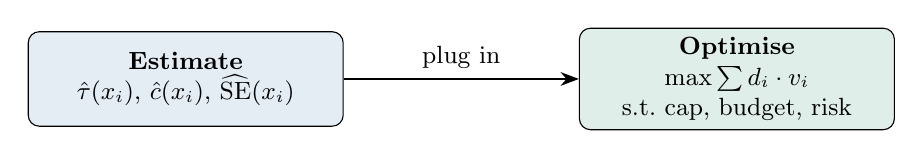
\begin{tikzpicture}[
    block/.style={draw, rounded corners, minimum width=4cm, minimum height=1.2cm, font=\small, align=center},
]
\node[block, fill=noteblue!12] (est) at (0,0) {\textbf{Estimate}\\$\hat{\tau}(x_i)$, $\hat{c}(x_i)$, $\widehat\SE(x_i)$};
\node[block, fill=sbgreen!12] (opt) at (7,0) {\textbf{Optimise}\\$\max \sum d_i \cdot v_i$\\s.t.\ cap, budget, risk};
\draw[tarrow] (est) -- (opt) node[midway, above, font=\small]{plug in};
\end{tikzpicture}
\end{center}

\pause
\bigskip

\begin{itemize}
    \item The \textbf{estimate} step is where causal inference lives: $\hat\tau$ needs the experiment; $\hat c$ needs only prediction.
    \item The \textbf{optimise} step is where the business lives: its constraints decide which errors in $\hat\tau$ matter.
    \item Plugging in treats estimates as truth. The safety margin and the conservative rule are the two places today where uncertainty was put back.
\end{itemize}

\small \textbf{The optimiser cannot tell supported inputs from extrapolated ones.} If the test had no low-spend executive controls, a model would still print $\hat\mu_0 = 0.30$ for them --- and the list would treat that number as data. Check support (M3) before ranking.
\end{frame}

% [CARRIED VERBATIM from old-decks/lecture06.tex:987]
\begin{frame}{SUTVA and Its Limits}
 
Everything today assumes \textbf{SUTVA}: each customer's treatment effect is independent of who else is treated.
 
\bigskip
 
This can fail at the coffee chain:
\begin{itemize}
    \item \textbf{Positive spillover:} a notified customer tells a friend about the seasonal drink.
    \item \textbf{Negative spillover:} a promotion at one store shifts demand from nearby stores.
    \item \textbf{Capacity interaction:} targeting too many customers near the same store causes congestion (capacity: see the notes).
\end{itemize}
 
\pause
\bigskip
 
When interference is present, the optimal policy depends on the \emph{entire assignment vector}, not just individual CATEs. Individual-level CATE targeting is an approximation when spillovers exist.
 
\end{frame}

% ====================================================================
\begin{frame}{The Progressive Ladder}

\begin{center}
\small
\begin{tabular}{p{4.5cm}p{4cm}p{4cm}}
\toprule
\textbf{Problem} & \textbf{Decision rule} & \textbf{What it adds} \\
\midrule
Free notification & $\hat{\tau}(x) > 0$ & Baseline \\[0.3em]
Opt-out cost (uniform) & $\hat{\tau}(x) > c/m$ & Threshold \\[0.3em]
Notification cap & Rank by $\hat{\tau}$, top $B$ & Competition \\[0.3em]
Customer-specific costs & $\hat{\tau} \cdot m > \hat{c}(x_i)$ & Two-model pipeline \\[0.3em]
Budget + heterog.\ costs & Rank by $r_i$, knapsack & Benefit-cost ratio; shadow price \\[0.3em]
Cost uncertainty & Safety margin $z_\alpha \hat{\sigma}_C$ & Budget buffer \\[0.3em]
Benefit uncertainty & Lower CI bound & Conservative targeting \\
\bottomrule
\end{tabular}
\end{center}

\bigskip

\small Capacity (a store's queue) and fairness constraints extend the ladder; they are in the notes, as reference material.
\end{frame}

% ====================================================================
\begin{frame}{Key Takeaways}

\begin{itemize}
    \item \spinestep{Estimand.} The net value of a list, $\sum_i d_i v_i$, under the constraints the business actually imposes. The effects $\hat\tau(x)$ never changed today; the list did.
    \item \spinestep{Identification.} The push test's coin identifies $\tau(x)$ cell by cell; transport to Q4 rests on \emph{same push, same coupon, same members}; the sum rests on no interference.
    \item \spinestep{Estimation, then decision.} Plug in $\hat\tau(x)$, $\hat c(x)$ and their uncertainty, then optimise. A cap makes members compete; the knapsack's marginal ratio prices the budget.
    \item \textbf{Prognostic variables return on the cost side.} Spending was irrelevant for $\hat\tau$; through $\hat c(x)$ it decides who is funded first.
    \item \textbf{Uncertainty on both sides.} A reserve protects the budget; a lower bound --- best on the value itself --- protects against noisy effects.
\end{itemize}
\end{frame}

% ====================================================================
\begin{frame}{Take-Home Targeting Core}

Done at home (30--45 minutes), submitted with Notebook 6 within 72 hours. Region 2, the push, the four cells above.

\bigskip

\begin{enumerate}\small
    \item Compute $v_i$ for each cell under uniform cost (\textyen 1.50) and under customer-specific cost. Rank the cells both ways.
    \item With \textyen 8{,}000 and no cap, solve the knapsack. Which cell is marginal, and what is $\lambda^*$?
    \item Add the 5\% overrun tolerance. How many marginal-cell members leave the list, and what does that cost in expected net?
    \item The forest's SE for analyst--high doubles to 6\%. Apply the conservative rule with $z = 1.645$. Does analyst--high stay on the list? What would you tell marketing?
    \item One paragraph to the CFO: the list, its expected net, and the two risks it does not cover.
\end{enumerate}

\bigskip

\textbf{Submit} with Notebook 6. Everything you need is on these slides; nothing is left to the lab.
\end{frame}

% ====================================================================
\begin{frame}{Lab 3: A Model That Calls Tools}

The simulated experimentation platform: a warehouse of experiment records, design documents and draft readouts. Fifty minutes.

\medskip

\begin{center}
\scriptsize
\begin{tabular}{rlp{8.6cm}}
\toprule
\textbf{Min} & \textbf{Slot} & \textbf{Task} \\
\midrule
5  & Task and specification & The question: \emph{``Did experiment E-217 pay, and for whom?''} Specify two tools --- a read-only SQL query over the records, and the statistical functions you verified in Lab 1. \\
10 & Demonstration & A model choosing which tool to call, reading the result, and calling again. \\
25 & Build & Wire the two tools; have the model answer the question from the records. Log every call. \\
7  & Verify & Check the model's numbers against your own query and your Lab 1 estimator. Did it use the right unit, the right arms, the right window? \\
3  & Interpret & One sentence: the first place the model would have gone wrong without the log. \\
\bottomrule
\end{tabular}
\end{center}

\small \textbf{Close:} a tool call returns a number; whether it is the \emph{right} number is still steps 1--3. This is the machinery of P4. Model, access and platform details: the lab handout and syllabus appendix.
\end{frame}

\end{document}
